\documentclass[a4paper, 14pt]{extarticle}

% Поля
%--------------------------------------
\usepackage{geometry}
\geometry{a4paper,tmargin=2cm,bmargin=2cm,lmargin=3cm,rmargin=1cm}
%--------------------------------------


%Russian-specific packages
%--------------------------------------
\usepackage[T2A]{fontenc}
\usepackage[utf8]{inputenc} 
\usepackage[english, main=russian]{babel}
%--------------------------------------

\usepackage{textcomp}

% Красная строка
%--------------------------------------
\usepackage{indentfirst}               
%--------------------------------------             


%Graphics
%--------------------------------------
\usepackage{graphicx}
\graphicspath{ {./images/} }
\usepackage{wrapfig}
%--------------------------------------

% Полуторный интервал
%--------------------------------------
\linespread{1.3}                    
%--------------------------------------

%Выравнивание и переносы
%--------------------------------------
% Избавляемся от переполнений
\sloppy
% Запрещаем разрыв страницы после первой строки абзаца
\clubpenalty=10000
% Запрещаем разрыв страницы после последней строки абзаца
\widowpenalty=10000
%--------------------------------------

%Списки
\usepackage{enumitem}

%Подписи
\usepackage{caption} 

%Гиперссылки
\usepackage{hyperref}

\hypersetup {
	unicode=true
}

%Рисунки
%--------------------------------------
\DeclareCaptionLabelSeparator*{emdash}{~--- }
\captionsetup[figure]{labelsep=emdash,font=onehalfspacing,position=bottom}
%--------------------------------------

\usepackage{tempora}

%Листинги
%--------------------------------------
\usepackage{listings}
\lstset{
  basicstyle=\ttfamily\footnotesize, 
  %basicstyle=\footnotesize\AnkaCoder,        % the size of the fonts that are used for the code
  breakatwhitespace=false,         % sets if automatic breaks shoulbd only happen at whitespace
  breaklines=true,                 % sets automatic line breaking
  captionpos=t,                    % sets the caption-position to bottom
  inputencoding=utf8,
  frame=single,                    % adds a frame around the code
  keepspaces=true,                 % keeps spaces in text, useful for keeping indentation of code (possibly needs columns=flexible)
  keywordstyle=\bf,       % keyword style
  numbers=left,                    % where to put the line-numbers; possible values are (none, left, right)
  numbersep=5pt,                   % how far the line-numbers are from the code
  xleftmargin=25pt,
  xrightmargin=25pt,
  showspaces=false,                % show spaces everywhere adding particular underscores; it overrides 'showstringspaces'
  showstringspaces=false,          % underline spaces within strings only
  showtabs=false,                  % show tabs within strings adding particular underscores
  stepnumber=1,                    % the step between two line-numbers. If it's 1, each line will be numbered
  tabsize=2,                       % sets default tabsize to 8 spaces
  title=\lstname                   % show the filename of files included with \lstinputlisting; also try caption instead of title
}
%--------------------------------------

%%% Математические пакеты %%%
%--------------------------------------
\usepackage{amsthm,amsfonts,amsmath,amssymb,amscd}  % Математические дополнения от AMS
\usepackage{mathtools}                              % Добавляет окружение multlined
\usepackage[perpage]{footmisc}
%--------------------------------------

%--------------------------------------
%			НАЧАЛО ДОКУМЕНТА
%--------------------------------------

\begin{document}

%--------------------------------------
%			ТИТУЛЬНЫЙ ЛИСТ
%--------------------------------------
\begin{titlepage}
\thispagestyle{empty}
\newpage


%Шапка титульного листа
%--------------------------------------
\vspace*{-60pt}
\hspace{-65pt}
\begin{minipage}{0.3\textwidth}
\hspace*{-20pt}\centering

\includegraphics[width=\textwidth]{emblem}
\end{minipage}
\begin{minipage}{0.67\textwidth}\small \textbf{
\vspace*{-0.7ex}
\hspace*{-6pt}\centerline{Министерство науки и высшего образования Российской Федерации}
\vspace*{-0.7ex}
\centerline{Федеральное государственное бюджетное образовательное учреждение }
\vspace*{-0.7ex}
\centerline{высшего образования}
\vspace*{-0.7ex}
\centerline{<<Московский государственный технический университет}
\vspace*{-0.7ex}
\centerline{имени Н.Э. Баумана}
\vspace*{-0.7ex}
\centerline{(национальный исследовательский университет)>>}
\vspace*{-0.7ex}
\centerline{(МГТУ им. Н.Э. Баумана)}}
\end{minipage}
%--------------------------------------

%Полосы
%--------------------------------------
\vspace{-25pt}
\hspace{-35pt}\rule{\textwidth}{2.3pt}

\vspace*{-20.3pt}
\hspace{-35pt}\rule{\textwidth}{0.4pt}
%--------------------------------------

\vspace{1.5ex}
\hspace{-35pt} \noindent \small ФАКУЛЬТЕТ\hspace{80pt} <<Информатика и системы управления>>

\vspace*{-16pt}
\hspace{47pt}\rule{0.83\textwidth}{0.4pt}

\vspace{0.5ex}
\hspace{-35pt} \noindent \small КАФЕДРА\hspace{50pt} <<Теоретическая информатика и компьютерные технологии>>

\vspace*{-16pt}
\hspace{30pt}\rule{0.866\textwidth}{0.4pt}
  
\vspace{11em}

\begin{center}
\Large {\bf Лабораторная работа № 3} \\
\large {\bf по курсу <<Численные методы линейной алгебры>>} \\
\large <<Реализация метода Гаусса c перестановками>>
\end{center}\normalsize

\vspace{8em}


\begin{flushright}
  {Студентка группы ИУ9-72Б Самохвалова П. С. \hspace*{15pt}\\
  \vspace{2ex}
  Преподаватель Посевин Д. П.\hspace*{15pt}}
\end{flushright}

\bigskip

\vfill
 

\begin{center}
\textsl{Москва 2023}
\end{center}
\end{titlepage}
%--------------------------------------
%		КОНЕЦ ТИТУЛЬНОГО ЛИСТА
%--------------------------------------

\renewcommand{\ttdefault}{pcr}

\setlength{\tabcolsep}{3pt}
\newpage
\setcounter{page}{2}

\section{Цель работы}\label{Sect::goal}

Реализовать три варианта метода Гаусса с перестановками и научиться
оценивать погрешность решения системы линейных уравнений для матриц
произвольной размерности.

\section{Задание}\label{Sect::task}

\begin{itemize}
    \item Реализовать метод Гаусса с перестановками по столбцам, по строкам, по столбцам и строкам одновременно для действительных квадратных матриц произвольной размерности n.
    \item Для проверки работоспособности алгоритмов необходимо использовать алгоритм тестирования задачи написанный в лабораторной работе №2 «Реализация метода Гаусса», который заключался в том, что мы заведомо определяем значения координат вектора x, данный вектор заведомо является решением уравнения A·х = b, вычисляем b путем прямого перемножения матрицы A на вектор x и далее производим поиск решения уравнения A·х = b тем или иным методом Гаусса, получая $x_{num}$, после чего производим сравнение полученного $x_{num}$ c заданным x, а также решением $x_{lib}$, полученным с использованием сторонней библиотеки выбранной студеном. При этом сравнение производится по Евклидовой норме разности вектора x - $x_{num}$ и x - $x_{lib}$.
    \item На защите лабораторной работы студент должен показать умение оценивать погрешность вычислений в зависимости от выполнения условия диагонального преобладания матрицы, умение сравнивать погрешности вычислений полученных методом Гаусса с перестановками по столбцам, по строкам, по столбцам и строкам одновременно. Понимать связь теории с практикой.
    \item Результат работы должен быть представлен в виде графиков зависимости абсолютной погрешности вычислений классическим методом Гаусса, методом Гаусса с перестановками по строкам, методом Гаусса с перестановками по столбцам, методом Гаусса с перестановками по столбцам и строкам, библиотечным методом от степени диагонального преобладания. Все графики должны быть построены на одной координатной плоскости. Напомним, что погрешность вычисления вектора x системы линейных алгебраических уравнений A·x=b тем или иным способом рассчитывается по Евклидовой норме разности точного решения и решения полученного соответствующим методом. Степень диагонального преобладания вычисляется, как максимальная разность по i между модулем диагонального элемента и суммы модулей вне диагональных элементов. Очевидно, что если значение степени диагонального преобладания положительна, то условие диагонального преобладания выполняется, в противном случае — не выполняется. Поэтому график должен быть построен как для отрицательных значений степени диагонального преобладания, так и для положительных.
\end{itemize}

\section{Практическая реализация}\label{Sect::code}

Исходный код программы представлен в листинге~\ref{lst:code1}.

\begin{lstlisting}[language={python},caption={Метод Гаусса},label={lst:code1}]
from num_methods import *
import random
import numpy as np
import copy
from matplotlib import pyplot as plt


def gauss_method(a, b):
    n = len(a)
    for i in range(n):
        for j in range(i + 1, n):
            c = - a[j][i] / a[i][i]
            for k in range(i, n):
                if k == i:
                    a[j][k] = 0
                else:
                    a[j][k] += c * a[i][k]
            b[j] += c * b[i]
    x = [0] * n
    for i in range(n - 1, -1, -1):
        x[i] = b[i]
        for j in range(n - 1, i, -1):
            x[i] -= x[j] * a[i][j]
        x[i] /= a[i][i]
    return x


def gauss_method_permutation_strings(a, b):
    n = len(a)
    for i in range(n):
        j_max = i
        for j in range(i + 1, n):
            if abs(a[j][i]) > abs(a[j_max][i]):
                j_max = j
        if j_max != i:
            for k in range(n):
                a[i][k], a[j_max][k] = a[j_max][k], a[i][k]
            b[i], b[j_max] = b[j_max], b[i]
        for j in range(i + 1, n):
            c = - a[j][i] / a[i][i]
            for k in range(i, n):
                if k == i:
                    a[j][k] = 0
                else:
                    a[j][k] += c * a[i][k]
            b[j] += c * b[i]
    x = [0] * n
    for i in range(n - 1, -1, -1):
        x[i] = b[i]
        for j in range(n - 1, i, -1):
            x[i] -= x[j] * a[i][j]
        x[i] /= a[i][i]
    return x


def gauss_method_permutation_columns(a, b):
    n = len(a)
    perm = [i for i in range(n)]
    for i in range(n):
        j_max = i
        for j in range(i + 1, n):
            if abs(a[i][j]) > abs(a[i][j_max]):
                j_max = j
        if j_max != i:
            for k in range(n):
                a[k][i], a[k][j_max] = a[k][j_max], a[k][i]
            perm[i], perm[j_max] = perm[j_max], perm[i]
        for j in range(i + 1, n):
            c = - a[j][i] / a[i][i]
            for k in range(i, n):
                if k == i:
                    a[j][k] = 0
                else:
                    a[j][k] += c * a[i][k]
            b[j] += c * b[i]
    x1 = [0] * n
    for i in range(n - 1, -1, -1):
        x1[i] = b[i]
        for j in range(n - 1, i, -1):
            x1[i] -= x1[j] * a[i][j]
        x1[i] /= a[i][i]
    x = [0] * n
    for i in range(n):
        x[perm[i]] = x1[i]
    return x


def gauss_method_permutation_strings_and_columns(a, b):
    n = len(a)
    perm = [i for i in range(n)]
    for i in range(n):
        j_max_str = i
        for j in range(i + 1, n):
            if abs(a[j][i]) > abs(a[j_max_str][i]):
                j_max_str = j
        j_max_col = i
        for j in range(i + 1, n):
            if abs(a[i][j]) > abs(a[i][j_max_col]):
                j_max_col = j
        if j_max_str != i or j_max_col != i:
            if j_max_str > j_max_col:
                for k in range(n):
                    a[i][k], a[j_max_str][k] = a[j_max_str][k], a[i][k]
                b[i], b[j_max_str] = b[j_max_str], b[i]
            else:
                for k in range(n):
                    a[k][i], a[k][j_max_col] = a[k][j_max_col], a[k][i]
                perm[i], perm[j_max_col] = perm[j_max_col], perm[i]
        for j in range(i + 1, n):
            c = - a[j][i] / a[i][i]
            for k in range(i, n):
                if k == i:
                    a[j][k] = 0
                else:
                    a[j][k] += c * a[i][k]
            b[j] += c * b[i]
    x1 = [0] * n
    for i in range(n - 1, -1, -1):
        x1[i] = b[i]
        for j in range(n - 1, i, -1):
            x1[i] -= x1[j] * a[i][j]
        x1[i] /= a[i][i]
    x = [0] * n
    for i in range(n):
        x[perm[i]] = x1[i]
    return x


def generate_matrix(n, v1, v2):
    return [[random.uniform(v1, v2) for i in range(n)] for j in range(n)]


def calculate_diagonal_predominance_degree(a):
    n = len(a)
    d = 0
    for i in range(n):
        s = 0
        for j in range(n):
            if i != j:
                s += abs(a[i][j])
        r = abs(a[i][i]) - s
        if i == 0:
            d = r
        elif r > d:
            d = r
    return d


def increase_diagonal_predominance_degree(a, k):
    n = len(a)
    a_new = copy.deepcopy(a)
    for i in range(n):
        s = 0
        for j in range(n):
            if i != j:
                s += abs(a[i][j])
        a_new[i][i] += s * k
    return a_new


def input_matrix():
    n = int(input())
    a = []
    b = []
    for i in range(n):
        l = list(map(int, input().split()))
        a.append(l)
    for i in range(n):
        b.append(int(input()))
    return a, b


plt.xlabel('Diagonal predominance degree')
plt.ylabel('Errors')


for n in [10, 50, 100]:

    a1 = generate_matrix(n, -10, 10)
    x = [i for i in range(1, n + 1)]

    k = [0, 0.5, 1, 1.5, 2]

    l = len(k)

    x_degrees = [0] * l
    y_gauss = [0] * l
    y_gauss_perm_str = [0] * l
    y_gauss_perm_col = [0] * l
    y_gauss_perm_str_and_col = [0] * l
    y_gauss_lib = [0] * l

    for i in range(l):

        a = increase_diagonal_predominance_degree(a1, k[i])
        d = calculate_diagonal_predominance_degree(a)

        b = mult_matr_vec(a, x)

        x_num = gauss_method(copy.deepcopy(a), copy.copy(b))
        x_num_perm_str = gauss_method_permutation_strings(copy.deepcopy(a), copy.copy(b))
        x_num_perm_col = gauss_method_permutation_columns(copy.deepcopy(a), copy.copy(b))
        x_num_perm_str_and_col = gauss_method_permutation_strings_and_columns(copy.deepcopy(a), copy.copy(b))
        x_lib = np.linalg.solve(a, b)

        norm_x_num = norm_vec(sub_vec(x, x_num))
        norm_x_num_perm_str = norm_vec(sub_vec(x, x_num_perm_str))
        norm_x_num_perm_col = norm_vec(sub_vec(x, x_num_perm_col))
        norm_x_num_perm_str_and_col = norm_vec(sub_vec(x, x_num_perm_str_and_col))
        norm_x_lib = norm_vec(sub_vec(x, x_lib))

        x_degrees[i] = d

        y_gauss[i] = norm_x_num
        y_gauss_perm_str[i] = norm_x_num_perm_str
        y_gauss_perm_col[i] = norm_x_num_perm_col
        y_gauss_perm_str_and_col[i] = norm_x_num_perm_str_and_col
        y_gauss_lib[i] = norm_x_lib

    plt.plot(x_degrees, y_gauss, color = "blue", label = "Gauss method classic")
    plt.plot(x_degrees, y_gauss_perm_str, color = "green", label = "Gauss method permutation strings")
    plt.plot(x_degrees, y_gauss_perm_col, color = "yellow", label = "Gauss method permutation columns")
    plt.plot(x_degrees, y_gauss_perm_str_and_col, color = "red", label = "Gauss method permutation strings and columns")
    plt.plot(x_degrees, y_gauss_lib, color = "black", label = "Gauss method library")

    plt.legend()

    plt.show()

\end{lstlisting}

\section{Результаты}\label{Sect::res}

Результаты работы программы представлены на рисунках~\ref{fig:img1}~--~\ref{fig:img3}.

\begin{figure}[!htb]
	\centering
	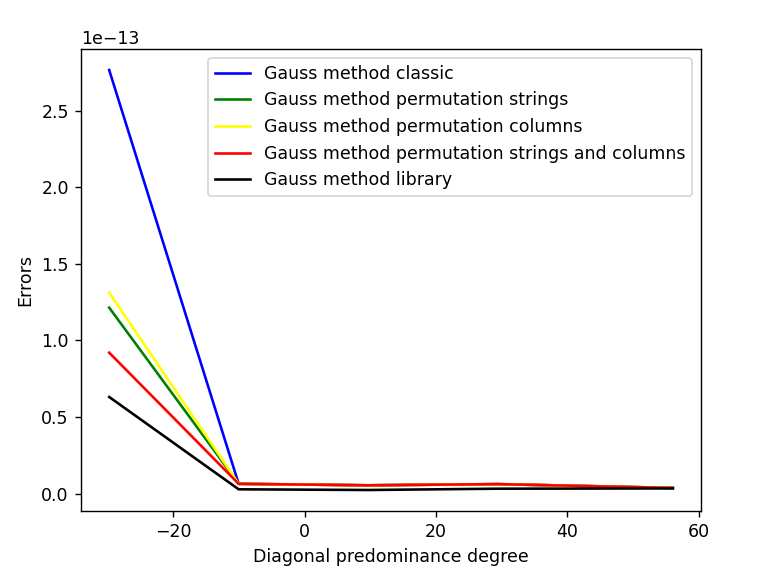
\includegraphics[width=0.8\textwidth]{img1}
\caption{Результат работы программы при n = 10}
\label{fig:img1}
\end{figure}

\begin{figure}[!htb]
	\centering
	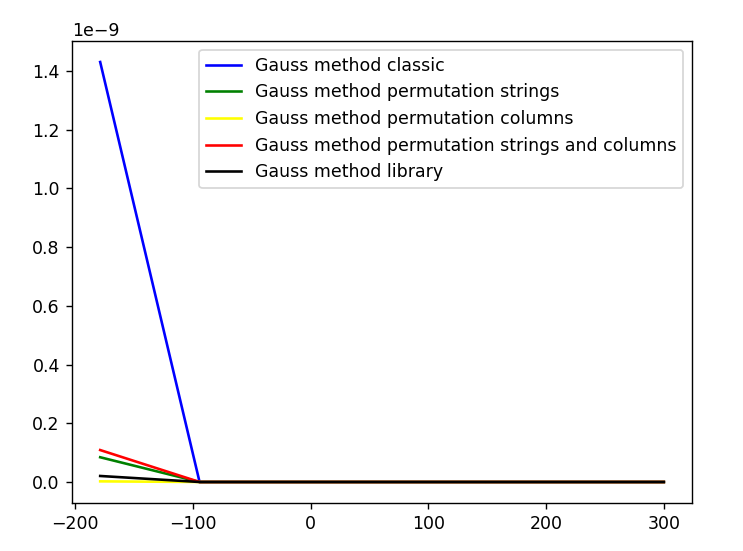
\includegraphics[width=0.8\textwidth]{img2}
\caption{Результат работы программы при n = 50}
\label{fig:img2}
\end{figure}

\begin{figure}[!htb]
	\centering
	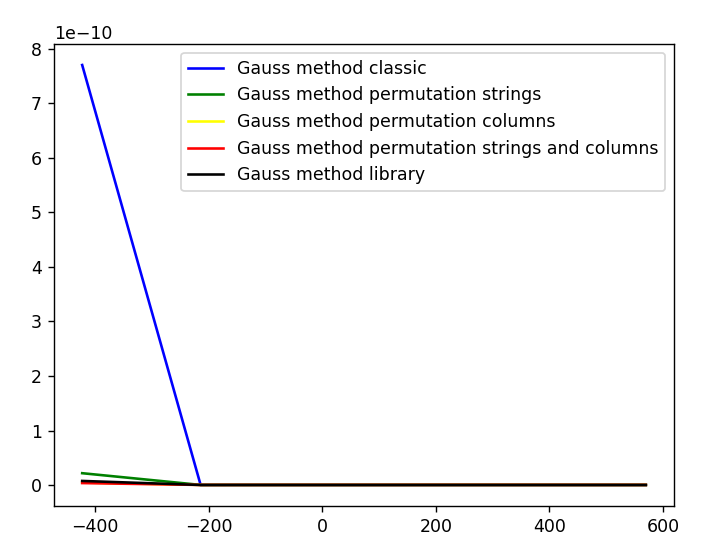
\includegraphics[width=0.8\textwidth]{img3}
\caption{Результат работы программы при n = 100}
\label{fig:img3}
\end{figure}

\section{Выводы}\label{Sect::conclusion}

В результате выполнения лабораторной работы были реализованы три варианта метода Гаусса с перестановками, была оценена погрешность решения системы линейных уравнений для матриц произвольной размерности.
\end{document}
